\chapter{Introdução}
\label{cha:introducao}


% Este documento apresenta considerações gerais e preliminares relacionadas 
% à redação de relatórios de Projeto de Graduação da Faculdade UnB Gama 
% (FGA). São abordados os diferentes aspectos sobre a estrutura do trabalho, 
% uso de programas de auxilio a edição, tiragem de cópias, encadernação, etc.

Um dos processos  que novos usurários Linux tem dificuldade em se adaptar é com a instalação de novas aplicações. Hoje é bem comum haver nas plataformas uma aplicação que centraliza a instalação das demais aplicações. Vista como uma loja em algumas plataformas, o gerenciador de aplicações tão comum nos dias atuais era a alguns anos um diferencial para sistemas Linux. Usurários Windows que se aventuravam nas terras do pinguim  tinham dificuldade para compreender que não precisavam acessar o site de um fabricante como a \textit{Adobe} para instalar o leitor de PDF, ou frequentar sites como \textit{Baixaki} para fazer o \textit{download} de aplicações diversas. Tudo o que precisavam era abrir o terminal e com alguns comandos o software era instalado de uma fonte confiável. A compreensão deste processo abria novas fronteiras para o novo usuário, que agora buscava expandir seu conhecimento e testar novas aplicações dentre as milhares que estavam ali disponível para ele gratuitamente. Obviamente que o processo de instalação e remoção de pacotes eventualmente torna-se dependente de uma ferramenta que possibilite realizar buscas por aplicações e filtragem das aplicações retornadas. E é aqui onde os novos usuários encontravam dificuldades em evoluir na busca por novos pacotes interessantes. Quando em linha de comando, as buscas por pacotes não se apresentam voltadas para usuários verdes ainda em comandos no terminal e sua ordenação é ainda menos intuitiva. Uma busca por \textit{"pdf"} no {\code apt} leva hoje a um resultado que, além de estourar o \textit{buffer} de linhas da janela do terminal, vem a apresentar o popular {\code evince} aproximadamente pela $14^a$ opção dentre os  pacotes disponíveis para instalação, dependendo das listas de repositórios adicionados na distribuição e qual gerenciador esta sendo usado.
Não o bastante, aplicações que pouco tem relação com leitores de \textit{pdf}, tais como o antivírus {\code clamav} ou o produtor de documentação {\code doxygen} aparecem antes do {\code evince} devido a ordenação alfabética.

\begin{figure}[h]
  \centering
	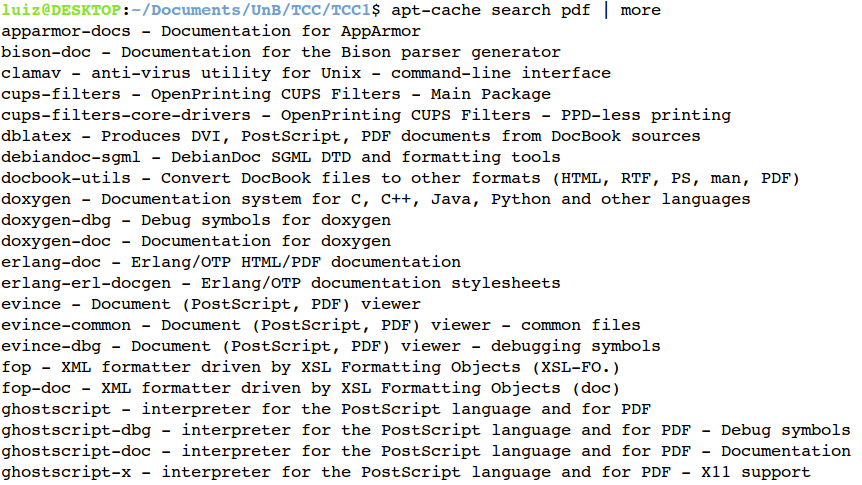
\includegraphics[width=0.6\textwidth]{figuras/search_pdf}
  \caption{Apresentação de resultados para \textit{pdf} usando o {\code apt-cache}}
  \label{fig:figuras_search_pdf}
\end{figure}

Dentre os diversos gerenciadores de pacotes utilizados atualmente para a instalação de pacotes em distribuições Linux, podemos apontar alguns que se destacam por virem já instalados de padrão nas distribuições mais comuns hoje e consequentemente são os mais  utilizados naquelas distribuições, como o {\code apt} ou o {\code yum}.

Porém, os principais gerenciadores possuem em comum o mesmo problema de ordenação de pacotes feitos em uma busca. A apresentação de resultados de busca não é personalizável, não permitindo classificar a listagem de pacotes por nome por exemplo, nem fazem \textit{matching} de aproximação  entre o pacote pesquisado e os possíveis candidatos. Desta forma a procura por um pacote do qual não se tenha o nome correto pode se tornar incrivelmente cansativa e desgastante, especialmente para um novo usuário Linux, que desconhece de ferramentas como o {\code grep, more} ou {\code  less}. 
